\section{1174021 - Muhammad Fahmi}
\subsection{Soal Teori}
\begin{enumerate}

	\item Jelaskan dengan ilustrasi gambar sendiri apa perbedaan antara vanilla GAN dan cGAN.
	\hfill\break
	Perbedaan antara vanilla GAN dan cGAN terdapat pada saat input proses generator, vanilla GAN memakai data noise yang di proses menjadi data fake, kalau cGAN memakai latent space atau label untuk generator. Untuk ilustrasi, lihat gambar berikut: 

	\begin{figure}[H]
	\centering
		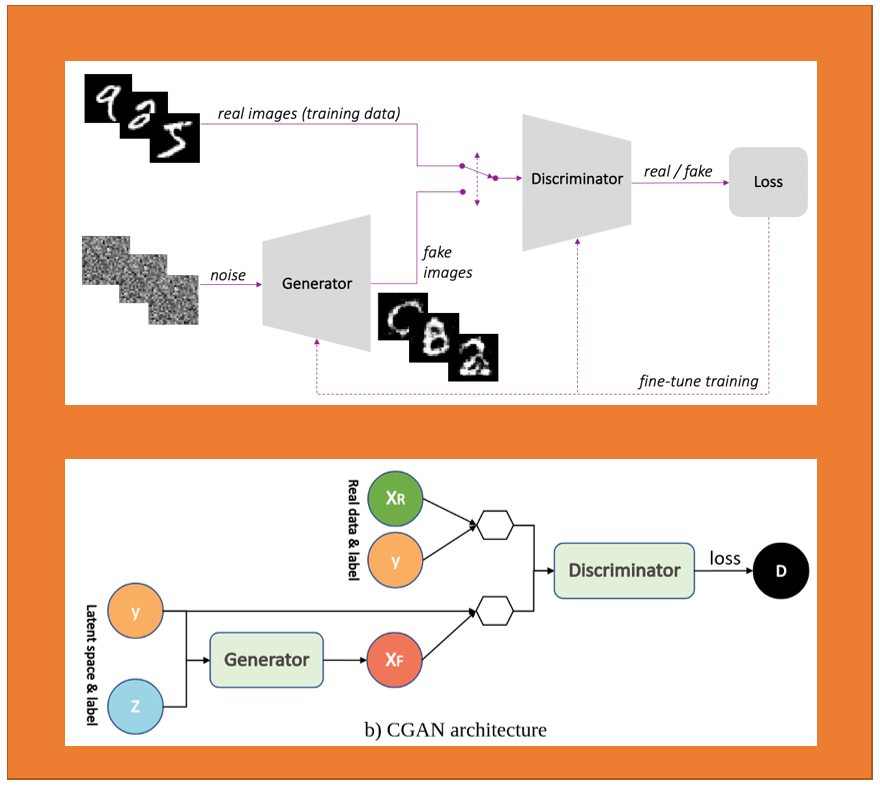
\includegraphics[width=4cm]{figures/1174021/tugas9/materi/teori1.PNG}
		\caption{Teori 1 }
	\end{figure}

	\item Jelaskan dengan ilustrasi gambar sendiri arsitektur dari Age-cGAN.

	\hfill\break
	Untuk arsitektur dari Age cGAN mempunyai 4 yaitu :
	\begin{itemize}
		\item Encoder
		\item FaceNet
		\item Generator
		\item Discriminator
	\end{itemize}
	Untuk ilustrasi, lihat gambar berikut: 

	\begin{figure}[H]
	\centering
		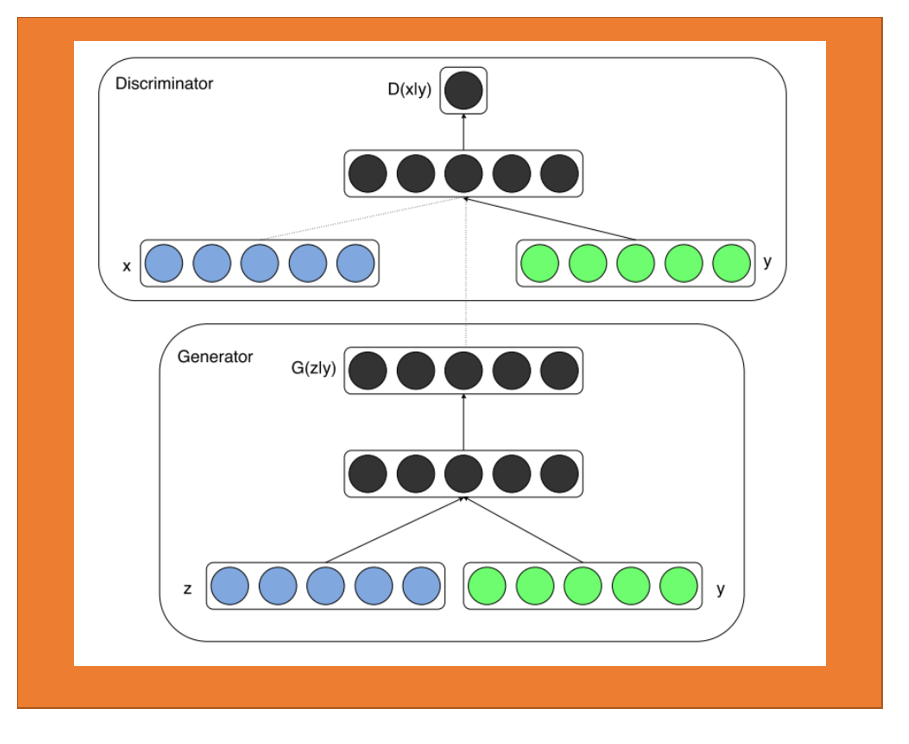
\includegraphics[width=4cm]{figures/1174021/tugas9/materi/teori2.PNG}
		\caption{Teori 2}
	\end{figure}
	
	\item Jelaskan dengan ilustrasi gambar sendiri arsitektur encoder network dari AgecGAN.

	\hfill\break
	Encoder mempelajari pemetaan terbalik dari gambar wajah input dan kondisi usia dengan vektor laten Z. Jaringan encoder menghasilkan vektor laten dari gambar input. Jaringan Encoder adalah CNN yang mengambil gambar dari dimensi (64, 64, 3) dan mengubahnya menjadi vektor 100 dimensi. Ada empat blok konvolusional dan dua lapisan padat. Setiap blok konvolusional memiliki lapisan konvolusional, diikuti oleh lapisan normalisasi batch, dan fungsi aktivasi kecuali lapisan konvolusional pertama.

	\begin{figure}[H]
	\centering
		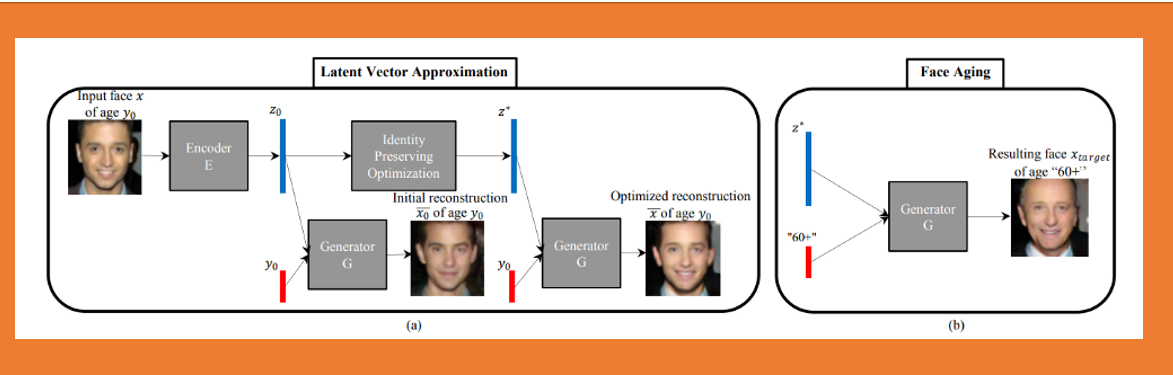
\includegraphics[width=4cm]{figures/1174021/tugas9/materi/teori345.PNG}
		\caption{Teori 3}
	\end{figure}

	\item Jelaskan dengan ilustrasi gambar sendiri arsitektur generator network dari AgecGAN.

	\hfill\break
	Generator dibutuhkan representasi tersembunyi dari gambar wajah dan vektor kondisi sebagai input dan menghasilkan gambar. Generator adalah CNN dan dibutuhkan vektor laten 100 dimensi dan vektor kondisi y, dan mencoba menghasilkan gambar realistis dari dimensi (64, 64, 3). Generator memiliki lapisan padat, membingungkan, dan konvolusional. Dibutuhkan dua input satu adalah vektor noise dan yang kedua adalah vektor kondisi. Vektor kondisi adalah informasi tambahan yang disediakan untuk jaringan. Untuk Age-cGAN, ini akan menjadi age.

	\begin{figure}[H]
	\centering
		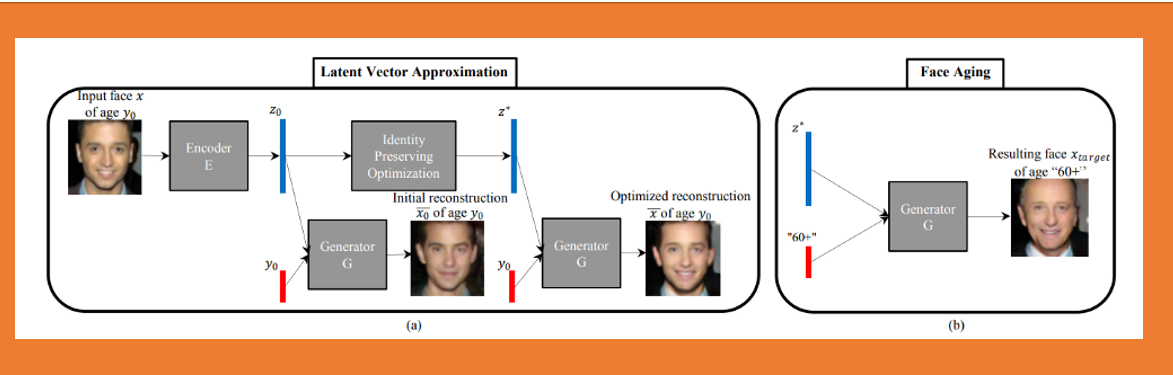
\includegraphics[width=4cm]{figures/1174021/tugas9/materi/teori345.PNG}
		\caption{Teori 4}
	\end{figure}

	\item Jelaskan dengan ilustrasi gambar sendiri arsitektur discriminator network dari Age-cGAN.
	\hfill\break
	Diskriminator mencoba membedakan antara gambar asli dan gambar palsu. Diskriminator adalah CNN dan memprediksi gambar yang diberikan adalah nyata atau palsu. Ada beberapa blok konvolusional. Setiap blok konvolusional berisi lapisan konvolusional yang diikuti oleh lapisan normalisasi batch, dan fungsi aktivasi, kecuali blok konvolusional pertama, yang tidak memiliki lapisan normalisasi batch.

	\begin{figure}[H]
	\centering
		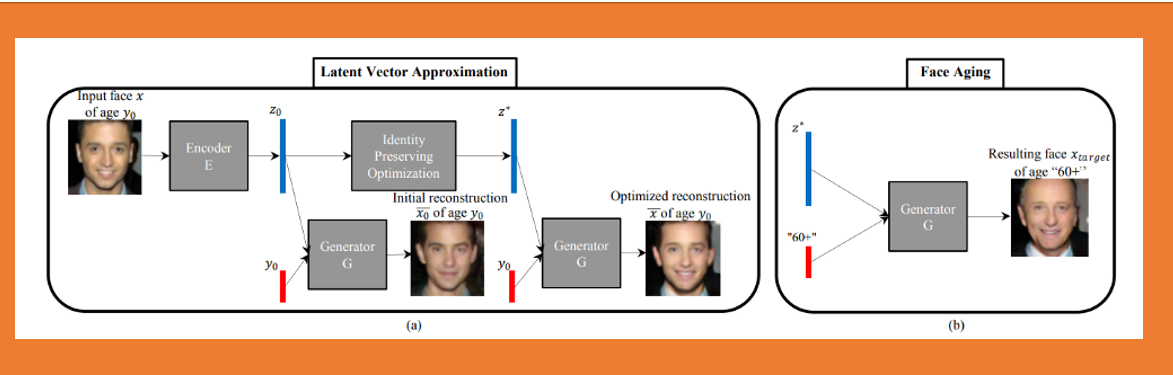
\includegraphics[width=4cm]{figures/1174021/tugas9/materi/teori345.PNG}
		\caption{Teori 5}
	\end{figure}

	\item Jelaskan dengan ilustrasi gambar apa itu pretrained Inception-ResNet-2 Model.
	\hfill\break
	Model Inception-ResNet v2 adalah model yang ciptakan untuk keperluan klasifikasi image dengan bobot di ImageNet.

	\begin{figure}[H]
	\centering
		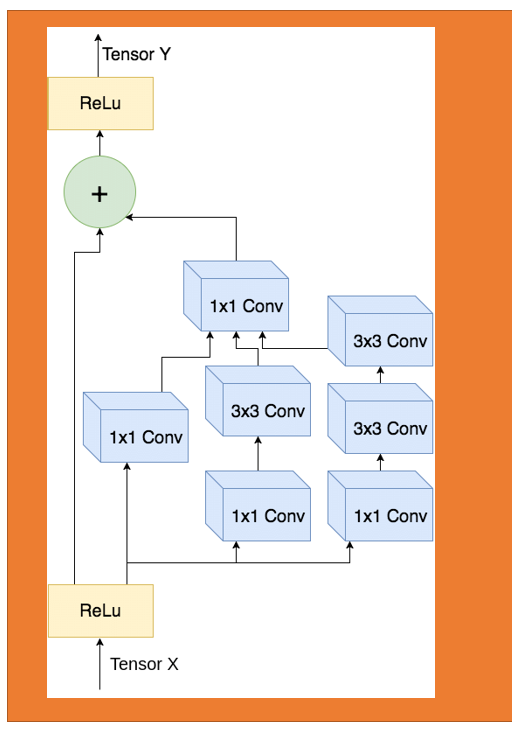
\includegraphics[width=4cm]{figures/1174021/tugas9/materi/teori6.PNG}
		\caption{Teori 6}
	\end{figure}

	\item Jelaskan dengan ilustrasi gambar sendiri arsitektur Face recognition network Age-cGAN.
	\hfill\break
	FaceNet: Ini adalah jaringan pengenalan wajah yang mempelajari perbedaan antara gambar input x dan gambar yang direkonstruksi x. FaceNet mengenali identitas seseorang dalam gambar yang diberikan. Model Inception, ResNet-50 atau Inception-ResNet-2 yang telah dilatih sebelumnya tanpa lapisan yang terhubung sepenuhnya dapat digunakan. Embedding yang diekstraksi untuk gambar asli dan gambar yang direkonstruksi dapat dihitung dengan menghitung jarak Euclidean dari embeddings.

	\begin{figure}[H]
	\centering
		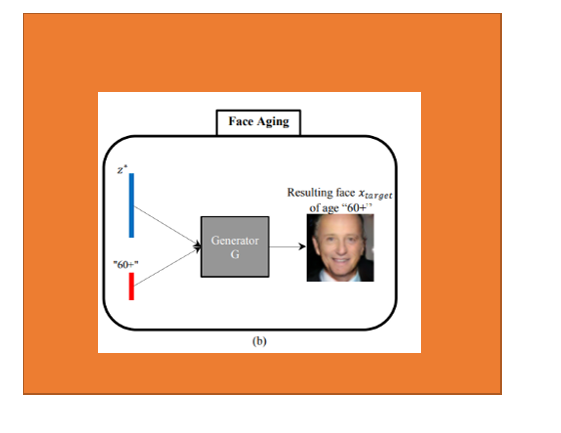
\includegraphics[width=4cm]{figures/1174021/tugas9/materi/teori7.PNG}
		\caption{Teori 7}
	\end{figure}

	%%CIE COPAS CIE %

	\item Sebutkan dan jelaskan serta di sertai contoh-contoh tahapan dari Age-cGAN.
	\hfill\break
	Untuk tahapan dari Age cGAN yaitu :
	\begin{itemize}
		\item Input
		\item Training
		\item Testing
	\end{itemize}

	\item Berikan contoh perhitungan fungsi training objektif
	\hfill\break
	Untuk penjelasan tersebut dijelaskan pada gambar dibawah ini :
	Fungsi obyektif training untuk training cGAN Dimana log D (x, y) adalah kerugian untuk model Diskriminator. log (1-D (G (x, y ’), y’)) adalah kerugian untuk model Generator. P (data) adalah distribusi dari semua gambar yang mungkin.

	\begin{figure}[H]
	\centering
		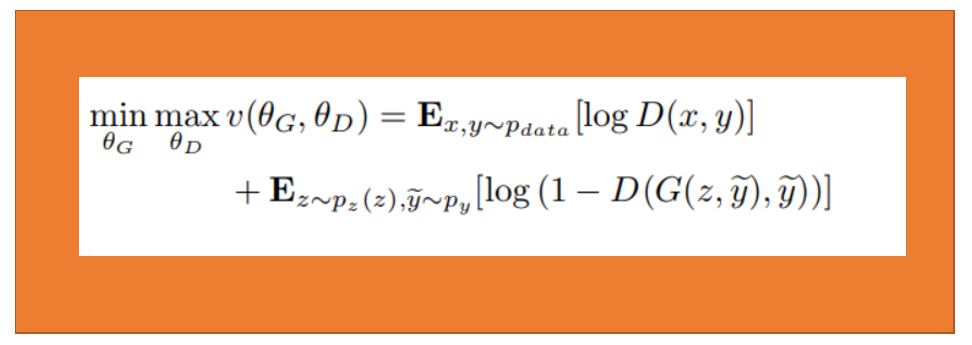
\includegraphics[width=4cm]{figures/1174021/tugas9/materi/teori9.PNG}
		\caption{Teori 9}
	\end{figure}

	\item Berikan contoh dengan ilustrasi penjelasan dari Initial latent vector approximation.
	\hfill\break

	Initial latent vector approximation: Encoder network training adakah seubah metode perkiraan awal vektor laten digunakan untuk memperkirakan vektor laten untuk mengoptimalkan rekonstruksi gambar wajah. Encoder adalah jaringan saraf yang mendekati vektor laten. Kami melatih jaringan encoder pada gambar yang dihasilkan dan gambar nyata. Setelah dilatih, jaringan encoder akan mulai menghasilkan vektor laten dari distribusi yang dipelajari. Fungsi tujuan pelatihan untuk melatih jaringan encoder adalah kehilangan jarak Euclidean.

	\item Berikan contoh perhitungan latent vector optimization
	\hfill\break

	\begin{figure}[H]
	\centering
		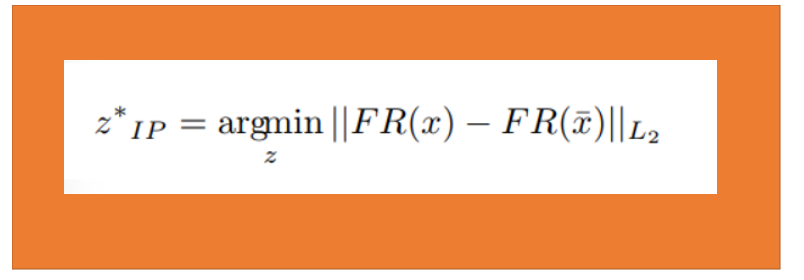
\includegraphics[width=4cm]{figures/1174021/tugas9/materi/teori11.PNG}
		\caption{Teori 11}
	\end{figure}
\end{enumerate}

\subsection{Praktek Program}
\begin{enumerate}
	\item Jelaskan bagaimana cara ekstrak file dataset Age-cGAN menggunakan google colab.
	\hfill\break

	\lstinputlisting[firstline=8, lastline=13]{src/1174021/tugas9/run.py}
	Kode di atas akan melakukan mount dan extract dataset.

	\begin{itemize}
		\item Login ke google colab menggunakan akun google
		\item Mount google drive
		\item Lakukan proses unzip melalui notebook python di google colab, unzip pakai codingan
		\item Selesai
	\end{itemize}

	\item Jelaskan bagaimana kode program bekerja untuk melakukan load terhadap dataset yang sudah di ekstrak, termasuk bagaimana penjelasan kode program perhitungan usia.
	\hfill\break
	\lstinputlisting[firstline=203, lastline=233]{src/1174021/tugas9/run.py}
	Kode di atas untuk load data dan melakukan fungsi perhitungan usia.
	
	\item Jelaskan bagaimana kode program The Encoder Network bekerja dijelaskan dengan bahawa awam dengan ilustrasi sederhana.
	\hfill\break
	\lstinputlisting[firstline=34, lastline=73]{src/1174021/tugas9/run.py}
	Encoder berfungsi untuk mempelajari pemetaan terbalik dari gambar wajah input dan kondisi usia dengan vektor laten Z.

	\item Jelaskan bagaimana kode program The Generator Network bekerja dijelaskan dengan bahawa awam dengan ilustrasi sederhana.
	\hfill\break
	\lstinputlisting[firstline=76, lastline=114]{src/1174021/tugas9/run.py}
	Generator network agar bekerja dengan baik dibutuhkan representasi tersembunyi dari gambar wajah dan vektor kondisi sebagai input dan menghasilkan gambar.

	\item Jelaskan bagaimana kode program The Discriminator Network bekerja dijelaskan dengan bahawa awam dengan ilustrasi sederhana.
	\hfill\break
	\lstinputlisting[firstline=124, lastline=155]{src/1174021/tugas9/run.py}
	Diskriminator mencoba untuk membedakan antara gambar asli dan gambar palsu.

	\item Jelaskan bagaimana kode program Training cGAN bekerja dijelaskan dengan bahasa awam dengan ilustrasi sederhana.
	\hfill\break
	\lstinputlisting[firstline=321, lastline=453]{src/1174021/tugas9/run.py}
	Proses training dengan load file .mat pada dataset, lalu epoch sebanyak 500 kali.

	\item Jelaskan bagaimana kode program Initial dan latent vector approximation bekerja dijelaskan dengan bahawa awam dengan ilustrasi sederhana.
	\hfill\break
	\lstinputlisting[firstline=459, lastline=592]{src/1174021/tugas9/run.py}
	Proses kerja nya dengan membuat model .h5, lalu load data dengan menghasilkan result.
	
\end{enumerate}

\subsection{Penanganan Error}
\begin{enumerate}
	\item ValueError
	\begin{figure}[H]
		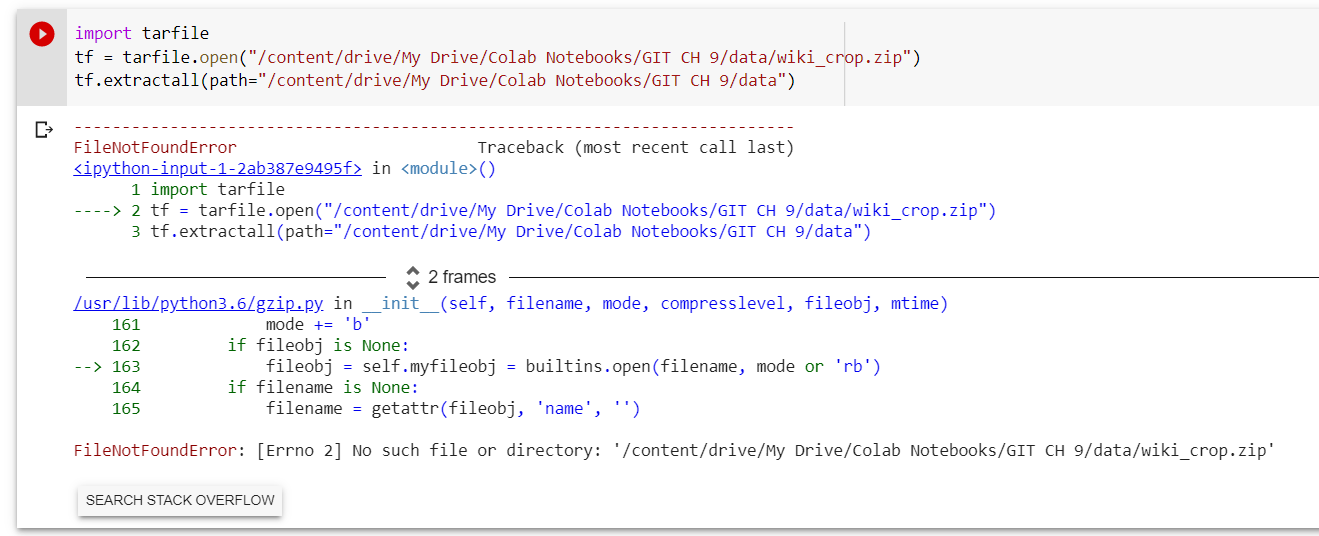
\includegraphics[width=4cm]{figures/1174021/tugas9/error/1.PNG}
		\centering
		\caption{FileNotFoundError}
	\end{figure}

	\item Cara Penanganan Error
	\begin{itemize}
		\item FileNotFoundError
		\hfill\break
		Error tersebut karena disebabkan gagal load dataset karena salah penamaan type file.
	\end{itemize}
\end{enumerate}

\subsection{Bukti Tidak Plagiat}
\begin{figure}[H]
\centering
	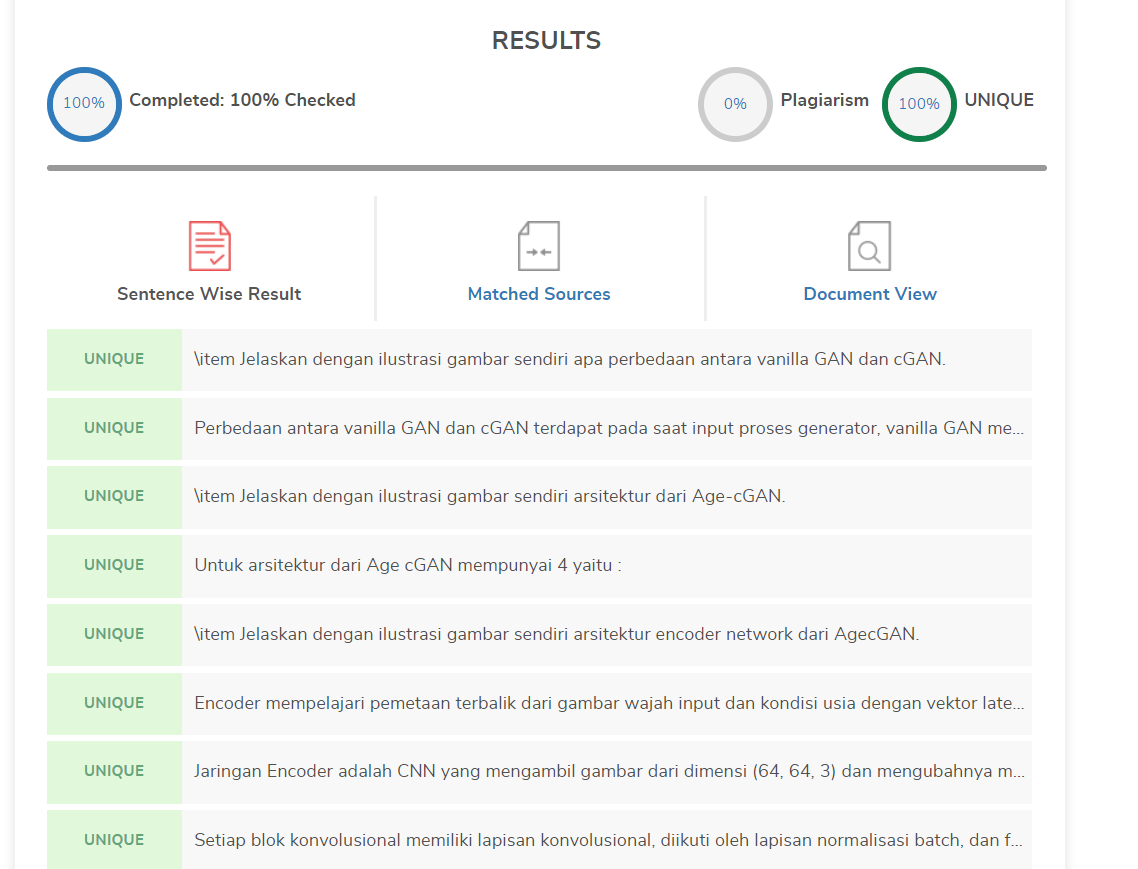
\includegraphics[width=4cm]{figures/1174021/tugas9/buktiplagiat/1.PNG}
	\caption{Bukti Tidak Melakukan Plagiat Chapter 9, CIE COPAS}
\end{figure}

